\section{X-ray diffraction}
One way where the 'Von Laue-Bragg' condition can be observed is in x-ray diffraction. The 'Von Laue-Bragg' condition states that an inciding electron is or scattered or stays unscattered when colliding with a crystal. This scattering is elastic thus the amplitude of the wave function does not change. This is illustrated in figure \ref{fig:vonlaue}.
\begin{figure}[b]
    \centering
    \begin{tikzpicture}
        \draw[->, black]	node[left] {$e^-$}(0, 0) to node[above]{incident} node[below]{$\vec{k}$} (2, 0);

        \draw[black] plot [smooth cycle] coordinates {(2.6, 0) (3.2, 0.6) (2.9, 0.7) (3.5, 1) (4.2, 0.9) (4.5, -0.3) (3.9, -0.2) (3.5, -0.7)} node [above=5mm, size=1pt]{CRYSTAL};

        \draw[->, black]	(5, 0.2) to node[above]{$\vec{k}'$}(6, 0.8) node[right=1mm]{$e^-$ (scattered)};
		\draw[->, black]	(5, 0) to node[below]{$\vec{k}$}(6, 0) node[right=1mm]{$e^-$ (unscattered)};
    \end{tikzpicture}
    \caption{X-ray diffraction on a lattice}
    \label{fig:vonlaue}
\end{figure}
Becuase the scattering is elastic we can state the following, define the wave as $e^{i\vec{k}\cdot\vec{r}}$:
\begin{align}
	E(\vec{k}) &= \frac{\hbar^2k^2}{2m}\\
	&= E(\vec{k}')\\
	&= \frac{\hbar^2k'^2}{2m}\\
	&\Rightarrow \abs{\vec{k}} = \abs{\vec{k}'}
\end{align}
One way of figuring out if an electron is scattered is to use the Fermi golden rule.

\section{Fermi golden rule} \label{sec:fermi}
\dfn{The fermi golden rule}{The fermi golden rule states that ($\tau_{\vec{k} \rightarrow \vec{k}'}$ is the mean time to have a diffraction):
\begin{equation}
	\frac{1}{\tau_{\vec{k} \rightarrow \vec{k}'}} = \frac{2\pi}{\hbar}\abs{<\vec{k}|V(\vec{r})|\vec{k}'>}^2\delta(E(\vec{k}) - E(\vec{k}'))
\end{equation}
}
We will look a bit further into this equation. We know that $V(\vec{r})=$ a periodic potential field of the crystal. Then
\begin{align}
	<\vec{k}|V(\vec{r})|\vec{k}'> \quad &= \int_{V}^{}d\vec{r}\frac{1}{\sqrt{V}}e^{i\vec{k}\cdot\vec{r}}V(\vec{r})\frac{1}{\sqrt{V}}e^{-i\vec{k}\cdot\vec{r}} \label{eqn:constants}\\
	&= \frac{1}{V}\sum_{\vec{R}}^{}\int_{\text{unit cell}}^{}d\vec{r}V(\vec{r}+\vec{R})e^{i(\vec{k}-\vec{k}')\cdot(\vec{r}+\vec{R})} \label{eqn:periodicity}
\end{align}
Equation \ref{eqn:constants} has normalization constants $\frac{1}{\sqrt{V}}$. Furthermore, in equation \ref{eqn:periodicity} we exploit hte periodicity of $V(\vec{r})$ and translation symmetry (section \ref{sec:trans_symm}). When is this integral in equation \ref{eqn:periodicity} non-zero?
\begin{equation}
	\text{The integral is non-zero } \iff \vec{k} - \vec{k}' = \vec{G} \text{ (the reciprocal lattice vector)} \label{eqn:Bragg_condition}
\end{equation}
Equation \ref{eqn:Bragg_condition} states the Bragg condition, futher elaborated in section \ref{sec:bragg}. By symmetry, we can leave $\vec{R}$ out of equation \ref{eqn:periodicity}, we get:
\begin{align}
	<\vec{k}|V(\vec{r})|\vec{k}'> \quad &= \frac{1}{V}\sum_{\vec{R}}^{}\int_{\text{unit cell}}^{}d\vec{r}V(\vec{r}+\vec{R})e^{i(\vec{k}-\vec{k}')\cdot\vec{r}}\\
	&\qquad\text{where } \int_{\text{unit cell}}^{}d\vec{r}V(\vec{r}+\vec{R})e^{i\vec{G}\cdot\vec{r}} = \tilde{V}(\vec{G})\\
	&\qquad\text{with } V(\vec{r}) = \sum_{\vec{G}}^{}\tilde{V}(\vec{G})e^{i\vec{G}\cdot\vec{r}}\\
	\iff & e^{i\vec{G}\cdot\vec{r}} = 1
\end{align}
As we know from section \ref{sec:reciproc_space} if $\vec{G} (= \vec{k} - \vec{k}')$ is not a reciprocal lattice vector, $\tilde{V}(\vec{G}) = 0$. $\vec{G}$ must be a lattice vector. The condition \ref{eqn:Bragg_condition} is the von Laue condition for constructive scattering.\par
So if we have elastic scattering, than the wavevectors and wavelengths are the same:
\begin{align}
	\abs{\vec{k}} &= \abs{\vec{k}'} \label{eqn:elastic}\\
	\frac{2\pi}{\lamba} &= \frac{2\pi}{\lambda'}\\
	\iff \lambda &= \lambda'
\end{align}
If we have the same wavelength, this scattering introduces extra distance for different incoming waves, we can see that in figure \ref{fig:extradistance}. The extra distance is defined by:
\begin{align}
	& \frac{\vec{R}}{\abs{\vec{k}}}\cdot\vec{k} - \frac{\vec{R}}{\abs{\vec{k}}}\cdot\vec{k}' = n\lambda\\
	&\Rightarrow \vec{R}(\vec{k} - \vec{k}') = 2\pi n\\
	&\Rightarrow e^{i\vec{R}(\vec{k}-\vec{k}')} = 1
\end{align}
This leaves us with the Bragg condition (section \ref{sec:bragg}), we can concude that: \begin{equation} \vec{k} - \vec{k}' = \vec{G} \end{equation}
\begin{figure}
	\centering
	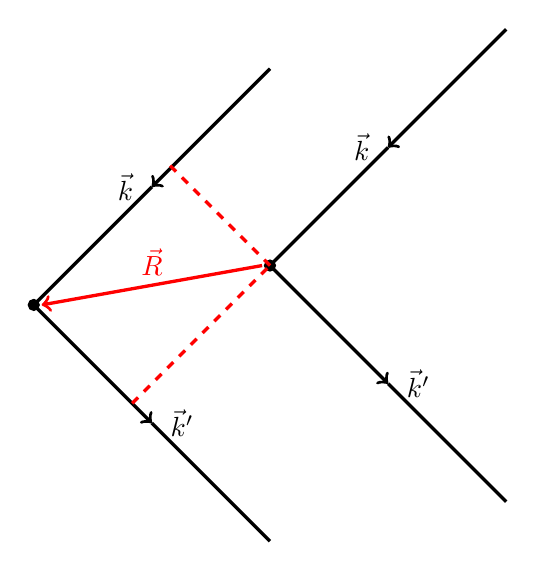
\begin{tikzpicture}
		\draw[->, black, very thick]	(3, 3) to (1.5, 1.5) node[left=1mm]{$\vec{k}$};
		\draw[-, black, very thick]		(1.5, 1.5) to (0, 0);

		\draw[->, black, very thick]	(6, 3.5) to (4.5, 2) node[left=1mm]{$\vec{k}$};
		\draw[-, black, very thick]		(4.5, 2) to (3, 0.5);

		\filldraw[black]	(0, 0) circle (2pt)
							(3, 0.5) circle (2pt);

		\draw[->, black, very thick]	(0, 0) to (1.5, -1.5) node[right=1mm]{$\vec{k}'$};
		\draw[-, black, very thick]		(1.5, -1.5) to (3, -3);

		\draw[->, black, very thick]	(3, 0.5) to (4.5, -1) node[right=1mm]{$\vec{k}'$};
		\draw[-, black, very thick]		(4.5, -1) to (6, -2.5);

		\draw[->, red, very thick] 	(2.9, 0.5) to (0.1, 0);
		\draw[red]		(1.5, 0.25) node[above]{$\vec{R}$};

		\draw[dashed, very thick, red]	(3, 0.5) to (1.7, 1.8);
		\draw[dashed, very thick, red]	(1.25, -1.25) to (3, 0.5);
	\end{tikzpicture}
	\caption{Extra distance for different wavevectors}
	\label{fig:extradistance}
\end{figure}

\section{Von Laue-Bragg condition} \label{sec:bragg}
As proven in section \ref{sec:fermi}, \begin{equation} \vec{k} - \vec{k}' = \vec{G} \end{equation}. We will rewrite this equation:
\begin{align}
	&\vec{k} - \vec{k}' = \vec{G}\\
	\iff&\vec{k}' = \vec{k} - \vec{G}\\
	\text{From eq. \ref{eqn:elastic}}\longrightarrow&\quad\abs{\vec{k}'}^2 = \abs{\vec{k}}^2 = k^2 = \abs{\vec{k} - \vec{G}}^2 = k^2 - 2\vec{k}\cdot\vec{G} + G^2\\
	\Rightarrow & z\vec{k}\cdot\vec{G} = G^2\\
	\iff& \vec{k}\cdot\frac{\vec{G}}{G} = \frac{G}{2}\\
	\iff&\vec{k}\cdot\vec{e}_{\vec{G}} = \frac{G}{2}\label{eqn:braggplane_derivation}
\end{align}
This means that the component of an incedent wave vector along the reciprocal lattice vector direction $G = \frac{\abs{\vec{G}}}{2}$. This is graphically represented in figure \ref{fig:halfdistance}. The dashed red line is a Bragg plane, this is generally defined by: \begin{equation} k\sin\theta = \frac{G}{2} \label{eqn:braggtheta}\end{equation}
\begin{figure}
	\centering
	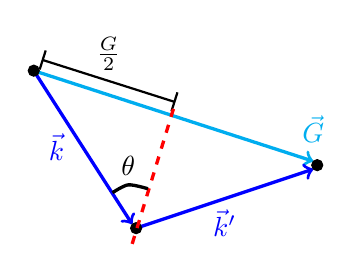
\begin{tikzpicture}
		\draw[->, cyan, very thick]	(0, 0) to (3.55, -1.15) node[above=1mm]{$\vec{G}$};
		\draw[->, blue, very thick]	(0, 0) to node[left=1mm]{$\vec{k}$} (1.25, -1.95);
		\draw[->, blue, very thick]	(1.3, -2) to node[below]{$\vec{k}'$} (3.55, -1.25);

		\filldraw[black]	(0, 0) circle (2pt)
							(1.3, -2) circle (2pt)
							(3.6, -1.2) circle (2pt);

		\draw[|-|, black, thick] (0.1, 0.14) to node[above]{$\frac{G}{2}$} (1.8, -0.4);
		\draw[dashed, red, very thick]	(1.25, -2.2) to (1.8, -0.4);

		\draw[black, very thick] plot [smooth] coordinates {(1, -1.55) (1.2, -1.45) (1.45, -1.5)};
		\draw[black]	(1.2, -1.45) node[above]{$\theta$};
	\end{tikzpicture}
	\caption{Drawing of the physical meaning of the Bragg condition}
	\label{fig:halfdistance}
\end{figure}
Furthermore, this bragg plane is derive from equation \ref{eqn:braggplane_derivation}. From the properites of reciprocal spaces, we know that (see equation \ref{eqn:braggplane_distande}):
\begin{align}
	& d = \frac{2\pi}{\vec{G}}\\
	& \text{with }\vec{G} = h\vec{b}_1 + k\vec{b}_2 + l\vec{b}_3 \\
	&\qquad\qquad\qquad \text{where h, k, l are Miller indices (section \ref{sec:latticeplanes})}
\end{align}
Now, form equation \ref{eqn:braggplane_distande} and equation \ref{eqn:braggtheta} we can derive an interference pattern. As we can see in figure \ref{fig:interference}, for normal scattering waves in a crystal lattice, Von Laue and the Bragg condition are the same. As we further also see, if the extra distance (marked with a dashed line) $d = n\lambda$, then there is no interference.
\begin{figure}
	\centering
	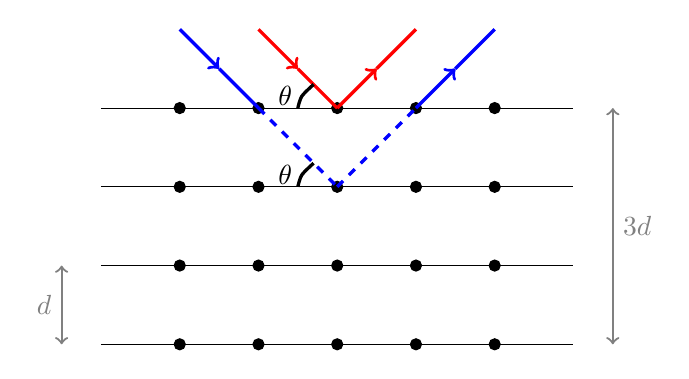
\begin{tikzpicture}
		\draw[-, black]	(-3, 0) to (3, 0)
						(-3, 1) to (3, 1)
						(-3, 2) to (3, 2)
						(-3, 3) to (3, 3);

		\filldraw[black]	(-2, 0) circle (2pt)
							(-1, 0) circle (2pt)
							(0, 0) circle (2pt)
							(1, 0) circle (2pt)
							(2, 0) circle (2pt)
							(-2, 1) circle (2pt)
							(-1, 1) circle (2pt)
							(0, 1) circle (2pt)
							(1, 1) circle (2pt)
							(2, 1) circle (2pt)
							(-2, 2) circle (2pt)
							(-1, 2) circle (2pt)
							(0, 2) circle (2pt)
							(1, 2) circle (2pt)
							(2, 2) circle (2pt)
							(-2, 3) circle (2pt)
							(-1, 3) circle (2pt)
							(0, 3) circle (2pt)
							(1, 3) circle (2pt)
							(2, 3) circle (2pt);

		\draw[->, blue, very thick]	(-2, 4) to (-1.5, 3.5);
		\draw[-, blue, very thick]	(-1.5, 3.5) to (-1, 3);
		\draw[dashed, blue, very thick]	(-1, 3) to (0, 2);
		\draw[dashed, blue, very thick]	(0, 2) to (1, 3);
		\draw[->, blue, very thick]	(1, 3) to (1.5, 3.5);
		\draw[-, blue, very thick]	(1.5, 3.5) to (2, 4);

		\draw[->, red, very thick]	(-1, 4) to (-0.5, 3.5);
		\draw[-, red, very thick]	(-0.5, 3.5) to (0, 3);
		\draw[->, red, very thick]	(0, 3) to (0.5, 3.5);
		\draw[-, red, very thick]	(0.5, 3.5) to (1, 4);

		\draw[<->, gray, thick]	(-3.5, 0) to node[left]{$d$} (-3.5, 1);
		\draw[<->, gray, thick]	(3.5, 0) to node[right]{$3d$} (3.5, 3);

		\draw[black, very thick] plot [smooth] coordinates {(-0.5, 3) (-0.45, 3.15) (-0.3, 3.3)};
		\draw[black, very thick] plot [smooth] coordinates {(-0.5, 2) (-0.45, 2.15) (-0.3, 2.3)};
		\draw[black]	(-0.45, 3.15) node[left]{$\theta$};
		\draw[black]	(-0.45, 2.15) node[left]{$\theta$};
	\end{tikzpicture}
	\label{Von Laue and Bragg interference pattern}
	\label{fig:interference}
\end{figure}
\ex{Von Laue - Bragg condition in 1D}{
For 1D, we can write the Von Laue condition as:
\begin{equation}
	\vec{k}\cdot\vec{G} = \frac{\abs{\vec{G}}^2}{2} \Rightarrow kG = \frac{G^2}{2} \label{eqn:braggpoints}
\end{equation}
We take the following 1D lattice:
\begin{center}
	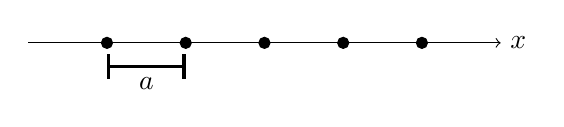
\begin{tikzpicture}
		\draw[->, black]	(-3, 0) to (3, 0) node[right]{$x$};

		\filldraw[black]	(-2, 0) circle (2pt)
							(-1, 0) circle (2pt)
							(0, 0) circle (2pt)
							(1, 0) circle (2pt)
							(2, 0) circle (2pt);

		\draw[|-|, black , very thick]	(-2, -0.3) to node[below]{$a$} (-1, -0.3);
	\end{tikzpicture}
\end{center}
With the following reciprocal 1D lattice and reciprocal vector $\vec{G} = \vec{b}$:
\begin{center}
	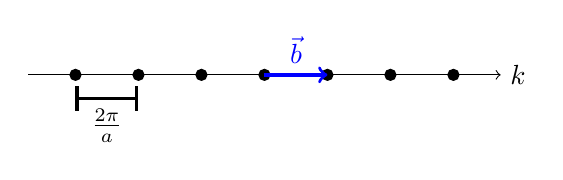
\begin{tikzpicture}
		\draw[->, black]	(-3, 0) to (3, 0) node[right]{$k$};

		\filldraw[black]	(-2.4, 0) circle (2pt)
							(-1.6, 0) circle (2pt)
							(-0.8, 0) circle (2pt)
							(0, 0) circle (2pt)
							(0.8, 0) circle (2pt)
							(1.6, 0) circle (2pt)
							(2.4, 0) circle (2pt);

		\draw[->, blue, very thick]		(0, 0) to node[above]{$\vec{b}$} (0.8, 0);

		\draw[|-|, black , very thick]	(-2.4, -0.3) to node[below]{$\frac{2\pi}{a}$} (-1.6, -0.3);
	\end{tikzpicture}
\end{center}
Then if we calculate the Bragg points, we get form equation \ref{eqn:braggpoints}:
\begin{equation}
	kb = \frac{b^2}{2} \Rightarrow k = \frac{b}{2}
\end{equation}
This results in the following Bragg points on the lattice:
\begin{center}
	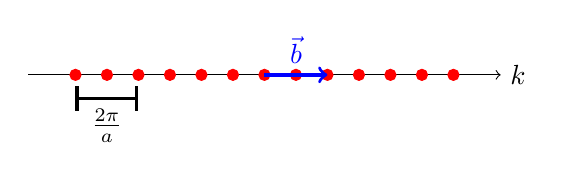
\begin{tikzpicture}
		\draw[->, black]	(-3, 0) to (3, 0) node[right]{$k$};

		\filldraw[red]	(-2.4, 0) circle (2pt)
							(-2, 0) circle (2pt)
							(-1.6, 0) circle (2pt)
							(-1.2, 0) circle (2pt)
							(-0.8, 0) circle (2pt)
							(-0.4, 0) circle (2pt)
							(0, 0) circle (2pt)
							(0.4, 0) circle (2pt)
							(0.8, 0) circle (2pt)
							(1.2, 0) circle (2pt)
							(1.6, 0) circle (2pt)
							(2, 0) circle (2pt)
							(2.4, 0) circle (2pt);

		\draw[->, blue, very thick]		(0, 0) to node[above]{$\vec{b}$} (0.8, 0);

		\draw[|-|, black , very thick]	(-2.4, -0.3) to node[below]{$\frac{2\pi}{a}$} (-1.6, -0.3);
	\end{tikzpicture}
\end{center}
}
\newpage

\section{The Brillouin Zone (BZ)} \label{sec:Brillouin}
\dfn{The frist Brillouin Zone}{The first Brillouin Zone is a Weigner-Sietz unit cell (section \ref{sec:weig_cell}) of the reciprocal lattice.\newline
For a 1D lattice, this becomes:
\begin{center}
	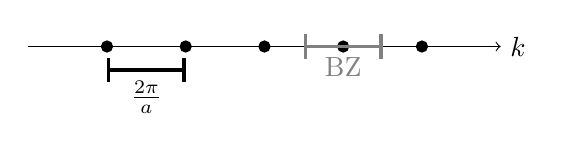
\begin{tikzpicture}
		\draw[->, black]	(-3, 0) to (3, 0) node[right]{$k$};

		\filldraw[black]	(-2, 0) circle (2pt)
							(-1, 0) circle (2pt)
							(0, 0) circle (2pt)
							(1, 0) circle (2pt)
							(2, 0) circle (2pt);

		\draw[|-|, black , very thick]	(-2, -0.3) to node[below]{$\frac{2\pi}{a}$} (-1, -0.3);

		\draw[|-|, gray, very thick]	(0.5, 0) to node[below]{BZ} (1.5, 0);
	\end{tikzpicture}
\end{center}
For a 2D lattice, the BZ (in gray) becomes:
\begin{center}
	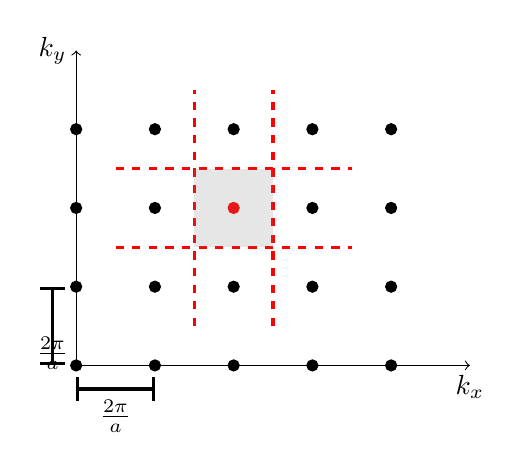
\begin{tikzpicture}
		\draw[->, black]	(-2, 0) to (3, 0) node[below]{$k_x$};
		\draw[->, black]	(-2, 0) to (-2, 4) node[left]{$k_y$};

		\filldraw[black]	(-2, 0) circle (2pt)
							(-1, 0) circle (2pt)
							(0, 0) circle (2pt)
							(1, 0) circle (2pt)
							(2, 0) circle (2pt)
							(-2, 1) circle (2pt)
							(-1, 1) circle (2pt)
							(0, 1) circle (2pt)
							(1, 1) circle (2pt)
							(2, 1) circle (2pt)
							(-2, 2) circle (2pt)
							(-1, 2) circle (2pt)
							(1, 2) circle (2pt)
							(2, 2) circle (2pt)
							(-2, 3) circle (2pt)
							(-1, 3) circle (2pt)
							(0, 3) circle (2pt)
							(1, 3) circle (2pt)
							(2, 3) circle (2pt);

		\filldraw[red]	(0, 2) circle (2pt);

		\draw[dashed, red, very thick]	(-0.5, 0.5) to (-0.5, 3.5);
		\draw[dashed, red, very thick]	(0.5, 0.5) to (0.5, 3.5);
		\draw[dashed, red, very thick]	(-1.5, 1.5) to (1.5, 1.5);
		\draw[dashed, red, very thick]	(-1.5, 2.5) to (1.5, 2.5);

		\draw[|-|, black , very thick]	(-2, -0.3) to node[below]{$\frac{2\pi}{a}$} (-1, -0.3);
		\draw[|-|, black , very thick]	(-2.3, 0) to node[below]{$\frac{2\pi}{a}$} (-2.3, 1);

		\fill[fill=gray, opacity=0.2] (-0.5, 1.5) to (-0.5, 2.5) to (0.5, 2.5) to (0.5, 1.5);
	\end{tikzpicture}
\end{center}
If $\vec{G}$ is defined on red dot, then the red dashed lines represent Bragg lines. The BZ is given in gray.
}
\subsection{Higher order BZ}
These higher order BZ are all the other zones limited by Bragg points (1D) / lines (2D) / planes (3D):
\begin{itemize}
	\item The first BZ is a set of points that can be reached without crossing other Bragg points / lines / planes.
	\item The second BZ is a set of points that can be reached by crossing Bragg points / lines / planes once. The second zone does not contain the lower order BZ.
	\item \dots
\end{itemize}
